\documentclass[aspectratio=169]{beamer}
\usefonttheme{serif}  % forza font serif classico anche in Beamer


% Tema minimale
\usetheme{default}
\usecolortheme{default}

% Sfondo bianco
\setbeamercolor{background canvas}{bg=white}

% Titolo slide
\setbeamercolor{frametitle}{fg=black,bg=white}
\setbeamerfont{frametitle}{size=\large,series=\bfseries}

% Rimuove simboli di navigazione
\setbeamertemplate{navigation symbols}{}
\setbeamertemplate{itemize item}{--}
\setbeamertemplate{footline}{
	\hfill\insertframenumber\hspace{0.4cm}\vspace{0.2cm}
}


% Titolo molto a sinistra
\setbeamertemplate{frametitle}{
  \vspace{0.4cm}
  \hspace*{-0.3cm}\insertframetitle
  \vspace{0.3cm}
}

\usepackage{lmodern}              % Latin Modern font
\usepackage{amsmath}              % miglior supporto matematico
\usepackage{graphicx}  % necessario per includere immagini
\setbeamerfont{math text}{family=\rmfamily}  % forza serif classico
\setbeamercolor{math text}{fg=black}        % colore nero
\usepackage{xcolor}
\usepackage{tikz}
\usetikzlibrary{positioning}



% Titolo della presentazione
\title{Quantum-enhanced LIDAR}
\subtitle{Esame di metà tesi}

\author{Federico Collé}
\institute{UNITO}

\begin{document}
% ===== SLIDE DI TITOLO =====
\begin{frame}[plain]
  \vfill
  \centering
  {\LARGE\bfseries Entanglement-based Quantum LiDAR\par}
  Esame di metà tesi\\
  \vspace{0.4cm}
  Federico Collé

  \vspace{0.8cm} % spazio prima delle immagini

  \begin{columns}[c]
    \column{0.45\textwidth}
    \centering
    \includegraphics[width=0.45\textwidth]{immagini/LOGO-UNITO_VERTICALE_COLORE-783119472.png}

    \column{0.45\textwidth}
    \centering
    \includegraphics[width=0.55\textwidth]{immagini/INRIM_logo-629767161.png}
  \end{columns}

  \vfill
\end{frame}

% ===== SLIDE  =====

\begin{frame}{Overview}
	\begin{itemize}
		\item Tecnologie quantistiche
		\item Protocollo di ranging
		\item Spontaneous Parametric Down Conversion
		\item Setup sperimentale
		\item Risultati
		\item Conclusioni e passi successivi
	\end{itemize}
\end{frame}


% ===== SLIDE  =====

\begin{frame}{Tecnologie quantistiche}

\begin{columns}
\column{0.45\textwidth}
    Tecnologie quantistiche: applicazioni tecnologiche legate a fenomeni prettamente quantistici.\\
    \vspace{0.3cm}
    Alcuni esempi:
\vspace{0.4cm}
\begin{itemize}
    \item Comunicazione quantistica
    \item Computazione quantistica
    \item Metrologia quantistica
    \item Quantum imaging \& sensing
\end{itemize}
\column{0.6\textwidth}
\begin{tikzpicture}
      % immagine "base"
  \node (A) {\includegraphics[width=0.5\textwidth]{immagini/ComputerQuantistico.jpg}};

  % immagini sovrapposte (spostate e sopra/sotto in base all'ordine)
  \node[above right=-6mm and -10mm of A] (B)
    {\includegraphics[width=0.5\textwidth]{immagini/QuantumMetrology.jpg}};

  \node[below right=-8mm and -6mm of A] (C)
    {\includegraphics[width=0.5\textwidth]{immagini/QuantumGhostImaging.jpg}};

  % questa la forzo "davanti" usando z-order (disegnandola per ultima) oppure:
  \node[above =-2mm of A] (D)
    {\includegraphics[width=0.5\textwidth]{immagini/QKD.jpg.jpg}};
  \node[below right=-7mm and -30mm of A] (E)
  	{\includegraphics[width=0.5\textwidth]{immagini/QuantumCommunication.png}};
\end{tikzpicture}
\end{columns}

\end{frame}

% ==============================

\begin{frame}{LiDAR}
LIDAR = LIght Detection And \textcolor{red}{Ranging}. \\
\vspace{0.2cm}

{
\centering
\includegraphics[width=0.7\linewidth]{immagini/schemaLIDAR2.png}
\par
}
\vspace{0.2cm}
È possibile migliorare il protocollo LiDAR sfruttando correlazioni quantistiche?

\end{frame}

%=======================================
\begin{frame}{Quantum LiDAR}
\begin{columns}
	\column{0.5\textwidth}
	Regime sotto studio:
	\begin{itemize}
		\item segnale basso ($\mu_0 \ll 1$)
		\item riflettività del target bassa ($k \ll 1$)
		\item background alto ($\mu_B \gg 1$)
	\end{itemize}
	$\rightarrow $ Situazione ostile
	\column{0.5\textwidth}
	\textbf{Obiettivo:} ridurre la probabilità di errore $p_{err} $ in
	\begin{itemize}
		\item \textit{Detection:} target presente o assente
		\item \textit{Ranging:} in quale time-bin è arrivato il ritorno
	\end{itemize}
\end{columns}
\vspace{1.5cm}		

\makebox[\textwidth][c]{%
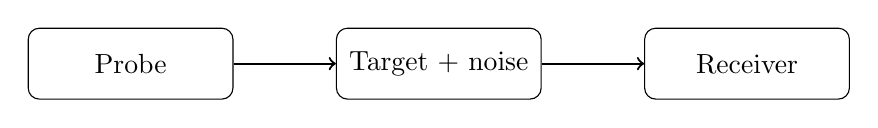
\begin{tikzpicture}[scale=0.55]
	% blocchi
	\node[draw, rounded corners, minimum width=2.6cm, minimum height=0.9cm] (src) {Probe};
	\node[draw, rounded corners, minimum width=2.6cm, minimum height=0.9cm, right=1.3cm of src] (tgt) {Target + noise};
	\node[draw, rounded corners, minimum width=2.6cm, minimum height=0.9cm, right=1.3cm of tgt] (rx) {Receiver};
	
	% frecce
	\draw[->, thick] (src) -- (tgt);
	\draw[->, thick] (tgt) -- (rx);
	

	

\end{tikzpicture}%
}


\end{frame}

%==================================

\begin{frame}{SPDC}
	\begin{columns}
		\column{0.5\textwidth}
		Spontaneous Parametric Down Conversion (SPDC):	\\
		\vspace{0.8cm}	
		{
			\centering
			\includegraphics[width=0.6\textwidth]{immagini/SPDCwikipedia.png}
			\par
		}
		\column{0.5\textwidth}
		{%
			\centering
			\includegraphics[width=1\textwidth]{immagini/diagramSPDC.png}
			\par
		}
		\vspace{0.5cm}	
		{
			\centering
			\includegraphics[width=0.6\textwidth]{immagini/consImpulsoSPDC.png}
			\par
		}
	\end{columns}
	
	
	
	$[\hat{n}_s - \hat{n}_i , \widehat{H}] = 0 \rightarrow$ $signal$ e $idler$ creati nello stesso momento.
	
	
\end{frame}

%=======================================

\begin{frame}{Quantum Target Detection (QTD)}
	
	\begin{columns}[T]
		\column{0.55\textwidth}
		
		\begin{itemize}
			\item \textbf{Probe:} stato $\rho_T$ con numero medio di fotoni $\mu_0$
			\item \textbf{Background:} stato $\rho_B$ con numero medio $\mu_B$
			\item \textbf{Target:} riflettività $k \ll 1$
			\item \textbf{Canale:} $\rho_k=\mathcal{E}_{k,\mu_B}(\rho_T)$
		\end{itemize}
				
		\vspace{0.25cm}
		\textcolor{red}{Binary hypothesis testing:}
		\begin{center}
			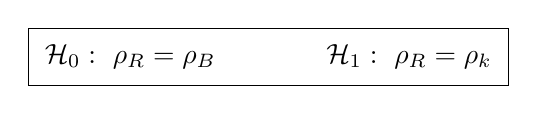
\begin{tikzpicture}
				\node[draw, inner sep=6pt] {
					$
					\mathcal{H}_0:\ \rho_R = \rho_B
					\qquad\qquad
					\mathcal{H}_1:\ \rho_R = \rho_k
					$
				};
			\end{tikzpicture}
		\end{center}
		
		
		\column{0.45\textwidth}
		\centering
		\includegraphics[width=0.95\textwidth]{immagini/DisegninoDetection.png}
		
	\end{columns}
	
\end{frame}

%==========================================

\begin{frame}{Quantum Target Detection (QTD)}
	\begin{columns}[T]
		\column{0.55\textwidth}
		Misura eseguita con stato a multi-copia $\rho_T^{\otimes L}$.\\
		Il canale $\mathcal{E}_{k,\mu_B}$ agisce indipendentemente su ogni copia.\\
		Per $L\to\infty$ vale il \textbf{Quantum Chernoff Bound} (QCB):
		\begin{equation*}
			p_{err}(\rho_0^{\otimes L},\rho_1^{\otimes L})
			\le \frac{1}{2}e^{-\xi_{QCB}L}
		\end{equation*}
		
		%\vspace{0.15cm}
		Con:
		\begin{equation*}
			\begin{aligned}
				\xi_{QCB}(\mathcal{H}_0,\mathcal{H}_1)
				&:= \max_{\alpha \in [0,1]} C_\alpha(\rho_0,\rho_1) \\
				C_\alpha(\rho_0,\rho_1)
				&:= -\log\!\big(\mathrm{Tr}[\rho_0^{\alpha}\rho_1^{1-\alpha}]\big)
			\end{aligned}
		\end{equation*}
		
		\column{0.45\textwidth}
		\centering
		\includegraphics[width=0.95\textwidth]{immagini/DisegninoDetectionTensorL.png}
	\end{columns}
	
%	\vspace{0.1cm}
	 $\xi_{QCB}$ = Chernoff information, $C_\alpha$ = $\alpha$-information.
	
\end{frame}

%===========================================

\begin{frame}{Quantum Target Ranging (QTR)}
	
	\begin{columns}[T]
		\column{0.48\textwidth}
		\centering
		\includegraphics[width=0.95\textwidth]{immagini/DisegninoRanging.png}
		
		\column{0.52\textwidth}
		Ranging = stima del tempo di volo.\\
		Asse dei tempi discretizzato in $m$ slot:
		
		\[
		\Delta t \ \Rightarrow\  m\ \text{time-bin}
		\qquad
		\Delta x = c\,\Delta t/2
		\]
		
		
		\textbf{Problema a $m$ ipotesi:}\\
		il target può cadere in uno degli $m$ slot.
		
		\vspace{0.2cm}
		\textcolor{red}{Problema a multi-hypothesis:}
		\begin{center}
			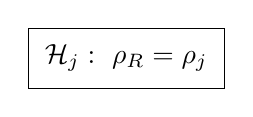
\begin{tikzpicture}
				\node[draw, inner sep=6pt] {
					$
					\mathcal{H}_j:\ \rho_R = \rho_j
					$
				};
			\end{tikzpicture}
		\end{center}
			
		
	\end{columns}
	
	\vspace{0.15cm}
	
		\[
		\rho_j := \rho_k^{(j)}\!\!\bigotimes_{i\neq j}^{m-1}\!\rho_B^{(i)}
		\quad
		\text{(solo nello slot $j$ c’è target+rumore)}
		\]
\end{frame}

%========================================

\begin{frame}{Quantum Target Ranging (QTR)}
	
\begin{columns}
	
	\column{0.48\textwidth}
	\centering
	\includegraphics[width=0.95\textwidth]{immagini/DisegninoRanging.png}
	
	\column{0.52\textwidth}
	Per $L \gg 1$ la probabilità di errore decresce esponenzialmente:
	\[
	p_{\mathrm{err}} \propto e^{-\xi^{(m)} L}
	\]

	\textbf{Asintoticamente} vale:
	\begin{equation*}
		\xi _{QCB}^{(m)}= \min_{i,j}\xi _{QCB}^{(2)}(\mathcal{H}_0,\mathcal{H}_1)
	\end{equation*}
	$\rightarrow $ errore dominato dalle due ipotesi più difficili da distinguere (time-bin vicini).\\
\end{columns}




\end{frame}

%==================================

\begin{frame}{Quantum Target Ranging (QTR)}
	
\begin{columns}
	\column{0.48\textwidth}
	\centering
	\includegraphics[width=0.95\textwidth]{immagini/DisegninoRanging.png}
	
	\column{0.52\textwidth}
	Siccome $\rho _j := \rho _k ^{(j)} \bigotimes_{i \ne j}^{m-1} \rho _B ^{(i)}$, è possibile confrontare due ipotesi qualsiasi, ad esempio:
	\begin{equation*}
		\rho_1 = \rho_k\otimes\rho_B\otimes\cdots
		\qquad
		\rho_2 = \rho_B\otimes\rho_k\otimes\cdots
	\end{equation*}
	Allora, per la Chernoff information:
	\begin{equation*}
		\xi_{TR} = \max_{\alpha\in[0,1]} C_\alpha(\rho_1,\rho_2)
		= 2\,C_{1/2}(\rho_k,\rho_B)
	\end{equation*}
	
	
\end{columns}
\vspace{0.5cm}
\centering
$\xi_{TD} := \max_{\alpha \in [0,1]}C_{\alpha}(\rho_B ,\rho_k) \ \rightarrow \ \xi_{TR}\ge \xi_{TD} \ \rightarrow \ \boxed{p_{err}^{TR}\le p_{err}^{TD}}  $
    
\end{frame}

%==================================

\begin{frame}{Misure Phase-Insensitive}
\textbf{Misura phase-insensitive} $\rightarrow$ si misura solo il \textbf{numero di fotoni}\\
\vspace{0.25cm}
	Per lo slot $j$ ottengo una distribuzione di conteggi:
\[
P_j(\vec n)=\mathrm{Tr}\!\left[\rho_j\,|\vec n\rangle\langle \vec n|\right],
\qquad
|\vec n\rangle=\bigotimes_i |n_i\rangle
\]
La best ranging performance è proporzionale a un set di distribuzioni di probabilità classiche
\begin{equation*}
	\{ \mathit{P}_1(\vec{n}),...,\mathit{P}_m(\vec{n})\}
\end{equation*}
 
        
\end{frame}

%==========================================

\begin{frame}{Misure Phase-Insensitive}
	

	\begin{columns}
		\column{0.5\textwidth}
			\textbf{Benchmark classico:} probe è stato coerente
		\[
		\xi_{\mathrm{coh}}
		= 2\mu_B + k\mu_0 - 2\sqrt{\mu_B}\sqrt{\mu_B+k\mu_0}
		\]
		
		\textbf{Probe quantistico:} $ \rho_Q = \rho_{\mathrm{TMSV}}^{\otimes R}$ \\
		$\rho_{\mathrm{TMSV}} = (| TMSV \rangle \langle TMSV|)  $\\
		$|TMSV \rangle=\sum_{n}c_n^{\mu_0}|n,n\rangle_{s.i}\langle n,n| $
		
		\vspace{0.2cm}
		\textbf{Quantum advantage:}
		\[
		\mathcal{Q}:=\frac{\xi_Q}{\xi_{\mathrm{coh}}}
		\]
		Limite empirico: $\mathcal{Q}_{emp} = 1+\frac{1}{\mu_0}$ ($k\ll 1$, $\mu_B\gg 1$).
		\column{0.5\textwidth}
		\centering
		\includegraphics[width=0.8\textwidth]{immagini/QvsKappa.png}
		\includegraphics[width=0.8\textwidth]{immagini/QvsMean.png}
	\end{columns}
	
	
\end{frame}

%==========================================

\begin{frame}{Setup sperimentale}

{
\centering
\includegraphics[width=1\textwidth]{immagini/SchemaSetupQuantistico.png}
\par
}
\vspace{0.25cm}
{\tiny BS: Beam Splitter   VA: Variable Attenuator   NLC: Non Linear Crystal   CWDM: Coarse Wavelength Division Multiplexing   DM: Dichroic Mirror   SNSPD: Superconducting Nanowire Single Photon detector}

\end{frame}

%============================================

\begin{frame}{Setup sperimentale}


{
\centering
\includegraphics[width=1\textwidth]{immagini/SchemaSetupClassico.png}
\par
}
\vspace{0.25cm}
{\tiny BS: Beam Splitter   VA: Variable Attenuator   NLC: Non Linear Crystal   CWDM: Coarse Wavelength Division Multiplexing   DM: Dichroic Mirror   SNSPD: Superconducting Nanowire Single Photon detector}
\end{frame}

%============================================

\begin{frame}{Analisi dei dati}
I conteggi dei dati vengono salvati in delle stringhe in base al tempo di arrivo.\\
\vspace{0.35cm}
{
\centering
\includegraphics[width=1\textwidth]{immagini/StringsCorrelationPicture.png}
\par}
Le stringhe vengono shiftate fino a trovare la posizione con il maggior coefficiente di Pearson, $C = \frac{\sigma_{XY}}{\sigma_X\sigma_Y}$.

\end{frame}

%============================================

\begin{frame}{Analisi dei dati}
Viene prima individuato il picco senza rumore, poi si aggiunge il rumore dopo.\\
\vspace{0.25cm}

\begin{columns}
    \column{0.33\textwidth}
    \centering
    \begin{figure}
        \includegraphics[width=1\textwidth]{immagini/piccoSenzaNoise.png}
        \caption{\footnotesize Picco senza rumore}
    \end{figure}

    \column{0.33\textwidth}
    \centering
    \begin{figure}
        \includegraphics[width=1\textwidth]{immagini/piccoConNoise.png}
        \caption{\footnotesize Picco con rumore}
    \end{figure}

    \column{0.33\textwidth}
    \centering
    \begin{figure}
        \includegraphics[width=1\textwidth]{immagini/piccoConTantoNoise.png}
        \caption{\footnotesize Picco con tanto rumore}
    \end{figure}
\end{columns}

\end{frame}

% ===========================================

\begin{frame}{Risultati}
    
\end{frame}

% ===== SLIDE  =====

\begin{frame}[plain]
  \vfill
  \centering
  {\LARGE\bfseries Grazie per l'attenzione\par}
  \vfill
\end{frame}

%============================================

\begin{frame}{SPDC}

Equazione di Maxwell in un dielettrico:
\begin{equation*}
    \vec{\nabla}^2 \vec{E} - \frac{1}{c^2} \frac{\partial^2 \vec{E}}{\partial t^2} = \frac{1}{\epsilon _0 c^2} \frac{\partial ^2 \vec{P}}{\partial t^2}
\end{equation*}
Dove  $\vec{P} = \vec{P} ^L + \vec{P} ^{NL}$ e  $  \vec{P}^{NL}_i = \epsilon _0 \sum _j \sum _k \chi _{ijk} ^{(2)} \cdot E_j E_k  $ .


\end{frame}

%===================================

\begin{frame}{SPDC}
	Spontaneous Parametric Down Conversion (SPDC): 
	\vspace{0.2cm}
	
	{%
		\centering
		\includegraphics[width=0.75\textwidth]{immagini/diagramSPDC.png}
		\par
	} 
	\vspace{0.2cm}
	Il fotone di pompa ($p$) entra nel cristallo non lineare, ne escono i fotoni signal ($s$) e idler ($i$).
	
\end{frame}

% =============================

\begin{frame}{SPDC}
	SPDC rispetta la conservazione di energia e impulso:
	\vspace{0.25cm}
	
	% ----- Prima equazione con immagine a destra -----
	\begin{columns}[]
		% Equazione a sinistra
		\column{0.5\textwidth}
		\begin{equation*}
			\hbar \omega_p = \hbar \omega_s + \hbar \omega_i
		\end{equation*}
		
		% Immagine a destra
		\column{0.55\textwidth}
		\centering
		\includegraphics[width=0.6\textwidth]{immagini/SPDCwikipedia.png}
	\end{columns}
	
	\vspace{0.1cm} % spazio tra le sezioni
	
	% ----- Seconda e terza equazione con immagine a sinistra -----
	\begin{columns}[]
		% Immagine a sinistra
		\column{0.55\textwidth}
		\centering
		\includegraphics[width=0.6\textwidth]{immagini/consImpulsoSPDC.png}
		
		% Equazioni a destra
		\column{0.5\textwidth}
		\begin{equation*}
			\vec{k}_p = \vec{k}_s + \vec{k}_i
		\end{equation*}
		
	\end{columns}
	
	\vspace{0.35cm}
	
	Inoltre vale $ \Delta \vec{k} = \vec{k}_p - \vec{k}_s - \vec{k}_i=\vec{0} $
	
\end{frame}

%=======SLIDE=========

\begin{frame}{SPDC}
	Il processo è descritto dall'Hamiltoniana:
	\begin{equation*}
		\widehat{H} = \sum _{k = p,s,i} \hbar \omega _k (\hat{n}_k + \frac{1}{2}) \ + \hbar g [\hat{a}_s ^{\dagger} \hat{a}_i ^{\dagger} \hat{a}_p + h.c.]
	\end{equation*}
	Dove $\hat{n}_k = \hat{a}_k ^{\dagger} \hat{a}_k $ e $h.c. =$ hermitiano congiunto. \\ 
	\vspace{0.3cm}
	
	Si dimostra facilmente che
	\begin{equation*}
		[\hat{n}_s + \hat{n}_i + 2\hat{n}_p , \widehat{H}] = 0
	\end{equation*}
	a mostrare come il fotone $p$ si trasforma nei due fotoni $s$ e $i$.
\end{frame}

% ===== SLIDE  =====

\begin{frame}{SPDC}
	L'efficienza della SPDC è molto bassa ($0.0004 \%$).\\
	Si può considerare $p$ come un campo classico, e il numero di fotoni $s$ e $i$ trascurabile rispetto a $p$:
	\begin{equation*}
		\hat{a}_p \longrightarrow \ a_p= v_p e^{-i\omega_p t} , \ \ \ \ \ \ \ \langle  \hat{n}_s(t) \rangle , \langle  \hat{n}_i(t) \rangle \ll \left| v_p \right| ^2
	\end{equation*}
	Allora:
	\begin{equation*}
		\widehat{H} = \sum _{k = p,s,i} \hbar \omega _k (\hat{n}_k + \frac{1}{2}) \ + \hbar g [\hat{a}_s ^{\dagger} \hat{a}_i ^{\dagger} v_p e^{-i \omega_p t} + h.c.]
	\end{equation*}
	Da cui segue
	\begin{equation*}
		[\hat{n}_s - \hat{n}_i , \widehat{H}] = 0
	\end{equation*}
	
	\vspace{0.1cm}
	La differenza $    \hat{n}_s(t) - \hat{n}_i(t) = \hat{n}_s(0) - \hat{n}_i(0)$ è una costante del moto: $s$ e $i$ si creano nello stesso momento.
	
	
	
\end{frame}

%=======================================

\begin{frame}{LiDAR}
	
	
	

	
	\begin{columns}[]
		% Immagine a sinistra
		\column{0.5\textwidth}
		Idea: sfruttare correlazioni quantistiche per migliorare la performance.
		\\ 
		\vspace{0.35cm}
		Vantaggio principalmente in situazioni ostili:
		rumore molto più intenso del segnale, riflettività del $target$ bassa.
		% Equazioni a destra
		\column{0.55\textwidth}
		\includegraphics[width=0.8\linewidth]{immagini/schemaLIDARdellaBotta.png}
		
	\end{columns}
	
\end{frame}

%=========================================

\begin{frame}{Misure Phase-Insensitive}
	
	Nel caso classico,
	\begin{equation*}
		\xi_{CB}^{(m)}=\min_{i.j}\xi_{CB}(\mathit{P}_i(\vec{n}),\mathit{P}_j(\vec{n})), \  \xi_{TR}^{cla} := \max_{\alpha\in [0,1]}\mathit{C}_{\alpha}^{cla}(P_BP_k,P_kP_B)=2\mathcal{B}_{TD}^{cla}
	\end{equation*}
	Da cui segue
	\begin{equation*}
		\xi_{coh}=2C_{1/2}(\mathcal{P}_k,\mathcal{P}_B)=2\mu_B
		+k\mu -2\sqrt{\mu_B}\sqrt{\mu_B+k\mu}  
	\end{equation*}
	Siamo in regime ottico: il background è monomodale e poissoniano, $P_B(n)=\mathcal{P}_{\mu_B}(n) $.\\
	Lo slot contenente sia il target sia il noise avrà la convoluzione delle due statistiche.
	
\end{frame}

%==========================================

\begin{frame}{Misure Phase-Insensitive}
	Rimane come definire la $Classic \ Chernoff \ Information$. Sarà uno stato coerente.
	\begin{equation*}
		\xi^{CLA}(p_0,p_1):= \max_{\alpha\in[0,1]}C_{\alpha}^{CLA}(p_0,p_1)=\max_{\alpha\in[0,1]}-\log(\sum_{\vec{n}}P_B(\vec{n})^{\alpha}P_k(\vec{n})^{1-\alpha}
	\end{equation*}
	E quindi per il TR ottengo
	\begin{equation*}
		\xi_{TR}^{CLA}:=\max_{\alpha\in[0,1]}C_{\alpha}^{CLA}(P_BP_k,P_kP_B)=2C_{1/2}^{CLA}(P_k,P_B)
	\end{equation*}
	E in generale
	\begin{equation*}
		\xi_{coh}=2C_{1/2}(P_k,P_B)=2\mu_B+k\mu-2\sqrt{\mu_B}\sqrt{\mu_B+k\mu}
	\end{equation*}
	
\end{frame}

%==========================================

\begin{frame}{Misure Phase-Insensitive}
	Il quantum probe è $\rho_Q= (| TMSV \rangle \langle TMSV|)^{\bigotimes R} , \ |TMSV \rangle=\sum_{n}c_n^{\mu_0}|n,n\rangle_{s.i}\langle n,n| $.\\
	C'è correlazione perfetta tra $signal$ e $idler$.\\
	Definisco il $Quantum \ Advantage$ come
	\begin{equation*}
		\mathcal{Q}:=\frac{\xi_Q}{\xi_{coh}}
	\end{equation*}
	
\end{frame}

%==========================================

\begin{frame}{Misure Phase-Insensitive}
	\begin{columns}
		\column{0.55\textwidth}
		\centering
		\includegraphics[width=0.8\textwidth]{immagini/QvsKappa.png}
		\column{0.55\textwidth}
		\includegraphics[width=0.8\textwidth]{immagini/QvsMean.png}
	\end{columns}
	Limite empirico, $\mathcal{Q}=1+\frac{1}{\mu} $ raggiunto per $k\ll 1 $ e $\mu_B \gg 1 $.\\
	
\end{frame}

%==========================================

\begin{frame}{Setup sperimentale}
	
	{
		\centering
		\includegraphics[width=0.7\textwidth]{immagini/SchemaSetupQuantistico.png}
		\par
	}
	%{\color{blue}\rule{\textwidth}{1pt}}
	\vspace{0.50cm}
	{
		\centering
		\includegraphics[width=0.7\textwidth]{immagini/SchemaSetupClassico.png}
		\par
	}
	\vspace{0.25cm}
	%{\tiny BS: Beam Splitter   VA: Variable Attenuator   NLC: Non Linear Crystal   CWDM: Coarse Wavelength Division Multiplexing   DM: Dichroic Mirror   SNSPD: Superconducting Nanowire Single Photon detector}
\end{frame}

%==========================================

\end{document}
